% chapters/03_framework.tex
\chapter{系统框架设计}

\section*{本章框架设计速览}

\begin{table}[H]
    \centering
    \begin{tabular}{p{0.18\textwidth}p{0.35\textwidth}p{0.37\textwidth}}
        \toprule
        \textbf{设计维度} & \textbf{核心决策} & \textbf{技术收益} \\
        \midrule
        核心抽象 & \texttt{BlockDevice} trait & 后端与 mapper 可互换、可堆叠 \\
        架构模式 & 装饰器 + 组合 & \texttt{Passthrough $\to$ Crypt $\to$ Verity} \\
        双目标 & 核心逻辑与平台无关 & 用户态验算法，内核态走真 BIO \\
        同步 & 用户态 \texttt{Mutex}；内核 \texttt{spin::Mutex} + 关抢占 & AES-NI 期间 XMM 不被打断 \\
        能力传播 & \texttt{TargetCapabilities} & 组合栈机密性/完整性/只读可静态汇总 \\
        可观测 & 原子计数器 + 阶段计时 & \texttt{/proc/dm-*-stats} 归因 \\
        \bottomrule
    \end{tabular}
\end{table}

\section{设计原则}

本项目的基本设计原则是使用统一的抽象来表示任何能够进行块级 I/O 的实体，并采用"分层"或"可组合"的架构，使加密和校验逻辑与底层存储介质完全解耦。核心设计原则包括：

\begin{enumerate}
    \item \textbf{统一抽象}：所有存储后端和映射器均实现同一个 \texttt{BlockDevice} trait，确保模块可互换、可堆叠；
    \item \textbf{双目标共享}：核心逻辑与平台无关，同时服务于用户态命令行工具（\texttt{dmctl}）和星绽内核（\texttt{aster-dm}）；
    \item \textbf{安全优先}：所有优化（缓存、缓冲池）遵循"先认证后使用"原则，不削弱安全边界；
    \item \textbf{可观测性内置}：关键路径嵌入原子计数器和阶段计时，支持性能归因和优化验证。
\end{enumerate}

这些原则共同确保了系统的可扩展性、可验证性和安全性——这正是 Device Mapper 作为可信存储底座的核心质量要求。

\section{核心抽象：BlockDevice Trait}

\texttt{BlockDevice} trait 是库中所有存储操作的基础接口，定义了用于读写固定大小数据块的同步接口。为了支持跨线程的并发访问并安全地集成到星绽内核或用户态工具中，该 trait 要求实现 \texttt{Send} 和 \texttt{Sync} 标记。Rust 通过这两个标记 trait 在编译期自动推导类型是否可安全地跨线程共享，无需开发者手动判断。

该 trait 定义如下：

\begin{lstlisting}[language=Rust, basicstyle=\ttfamily\small, breaklines=true]
pub trait BlockDevice: Send + Sync {
    fn block_size(&self) -> usize;
    fn num_blocks(&self) -> u64;
    fn read_block(&self, block_id: u64, buf: &mut [u8]) -> Result<()>;
    fn write_block(&self, block_id: u64, buf: &[u8]) -> Result<()>;
}
\end{lstlisting}

所有 I/O 方法均返回 \texttt{Result<()>}，其中错误被封装在 \texttt{DmError} 枚举中，涵盖无效块大小、无效块号、密钥错误、完整性违规等场景。这个 trait 的设计借鉴了 Linux 内核 \texttt{block\_device\_operations} 的职责分离思想，但通过 Rust 的类型系统提供了更强的安全性保证——任何不安全的跨线程访问在编译期就会被阻止。

在 Asterinas 内核中，该 trait 进一步映射到 \texttt{aster-block} 组件的 BIO 接口，从而支持真实的 VirtIO 块设备。

\section{可组合的映射器链模式}

该架构采用类似装饰器（Decorator）的设计模式。每个映射器（如 \texttt{DmCryptDevice} 和 \texttt{DmVerityDevice}）既实现了 \texttt{BlockDevice} trait，又在内部消费（包装）另一个实现了 \texttt{BlockDevice} 的对象，支持功能的任意堆叠与组合。

例如，一个典型的用户态栈可能是：

\begin{lstlisting}[language=Rust, basicstyle=\ttfamily\small, breaklines=true]
let file = FileBlockDevice::open("disk.img")?;
let crypt = DmCryptDevice::new(file, key)?;
let verity = DmVerityDevice::open(crypt, tree, root_hash)?;
\end{lstlisting}

在星绽内核中，这种组合通过 \texttt{DmDevice} 结构体实现，它根据 \texttt{DmTarget} 枚举（Passthrough、Crypt、Verity）分发 BIO 请求。由于每个 mapper 的下层是 \texttt{Arc<dyn BlockDevice>}，启动阶段可将 \texttt{rootfs\_verity.device} 指向已注册的 crypt mapper 名（如 \texttt{dm-crypt0}），或显式设置 \texttt{dm\_stack=crypt,verity}，从而形成与用户态相同的叠栈：\texttt{vdc $\to$ dm-crypt0 $\to$ dm-verity0}。验收脚本为 \texttt{scripts/run\_dm\_stack.sh}。

\section{核心模块分解}

项目被结构化为离散的模块，以清晰地分离密码学原语、数据结构和设备逻辑。整个 \texttt{dm} crate 约 3000 行 Rust 代码，\texttt{dmctl} 约 800 行；内核补丁 0001--0007 约 4000 行。不是两套互不相干的实现：用户态是算法与布局的安全网，内核态才是赛题交付物。模块划分如下：

\begin{table}[H]
    \centering
    \caption{核心模块职责划分与代码量}
    \begin{tabular}{p{0.16\textwidth}p{0.38\textwidth}p{0.10\textwidth}p{0.26\textwidth}}
        \toprule
        \textbf{模块} & \textbf{主要职责} & \textbf{约行数} & \textbf{关键实体} \\
        \midrule
        \texttt{block\_device} & 抽象与文件/内存后端 & 400 & \texttt{BlockDevice}, \texttt{FileBlockDevice}, \texttt{MemoryBlockDevice} \\
        \texttt{dm\_crypt} & AES-XTS 透明加密 & 350 & \texttt{DmCryptDevice}, \texttt{DmCryptTable} \\
        \texttt{dm\_verity} & 只读完整性 & 200 & \texttt{DmVerityDevice} \\
        \texttt{hash\_tree} & Merkle 构建与校验 & 150 & \texttt{HashTree} \\
        \texttt{sha256} & 纯 Rust SHA-256 & 120 & \texttt{sha256::sha256} \\
        \texttt{device\_mapper} & 链接与 \texttt{DmStackBuilder} & 180 & \texttt{PassthroughDevice}, \texttt{DmStackBuilder} \\
        \texttt{statistics} & I/O 与阶段归因 & 150 & \texttt{InstrumentedDevice}, \texttt{IoStatsSnapshot} \\
        \texttt{runtime} & 运行时 mapper / \texttt{dm\_ioctl} & 260 & \texttt{RuntimeMapper}, \texttt{DmControlDevice} \\
        \bottomrule
    \end{tabular}
\end{table}

\texttt{BlockDevice} 实现涵盖了多种后端场景：
\begin{itemize}
    \item \texttt{MemoryBlockDevice}：基于内存向量的设备，主要用于单元测试和易失性存储；
    \item \texttt{FileBlockDevice}：由宿主机文件系统上的文件支持的持久化设备，由 \texttt{dmctl} 工具使用；
    \item \texttt{PassthroughDevice}：将调用直接转发给内部设备的包装器，用于验证映射器链；
    \item \texttt{VirtioBlkAdapter}：（星绽移植版）将内核特定的块设备句柄适配到 \texttt{BlockDevice} 接口，位于 \texttt{aster-dm} 组件中。
\end{itemize}

\section{双目标架构：跨环境可移植性}

一个核心设计目标是：相同的逻辑同时服务于用户态演示和星绽内核。这是通过严格隔离环境特定代码来实现的。

\begin{figure}[H]
    \centering
    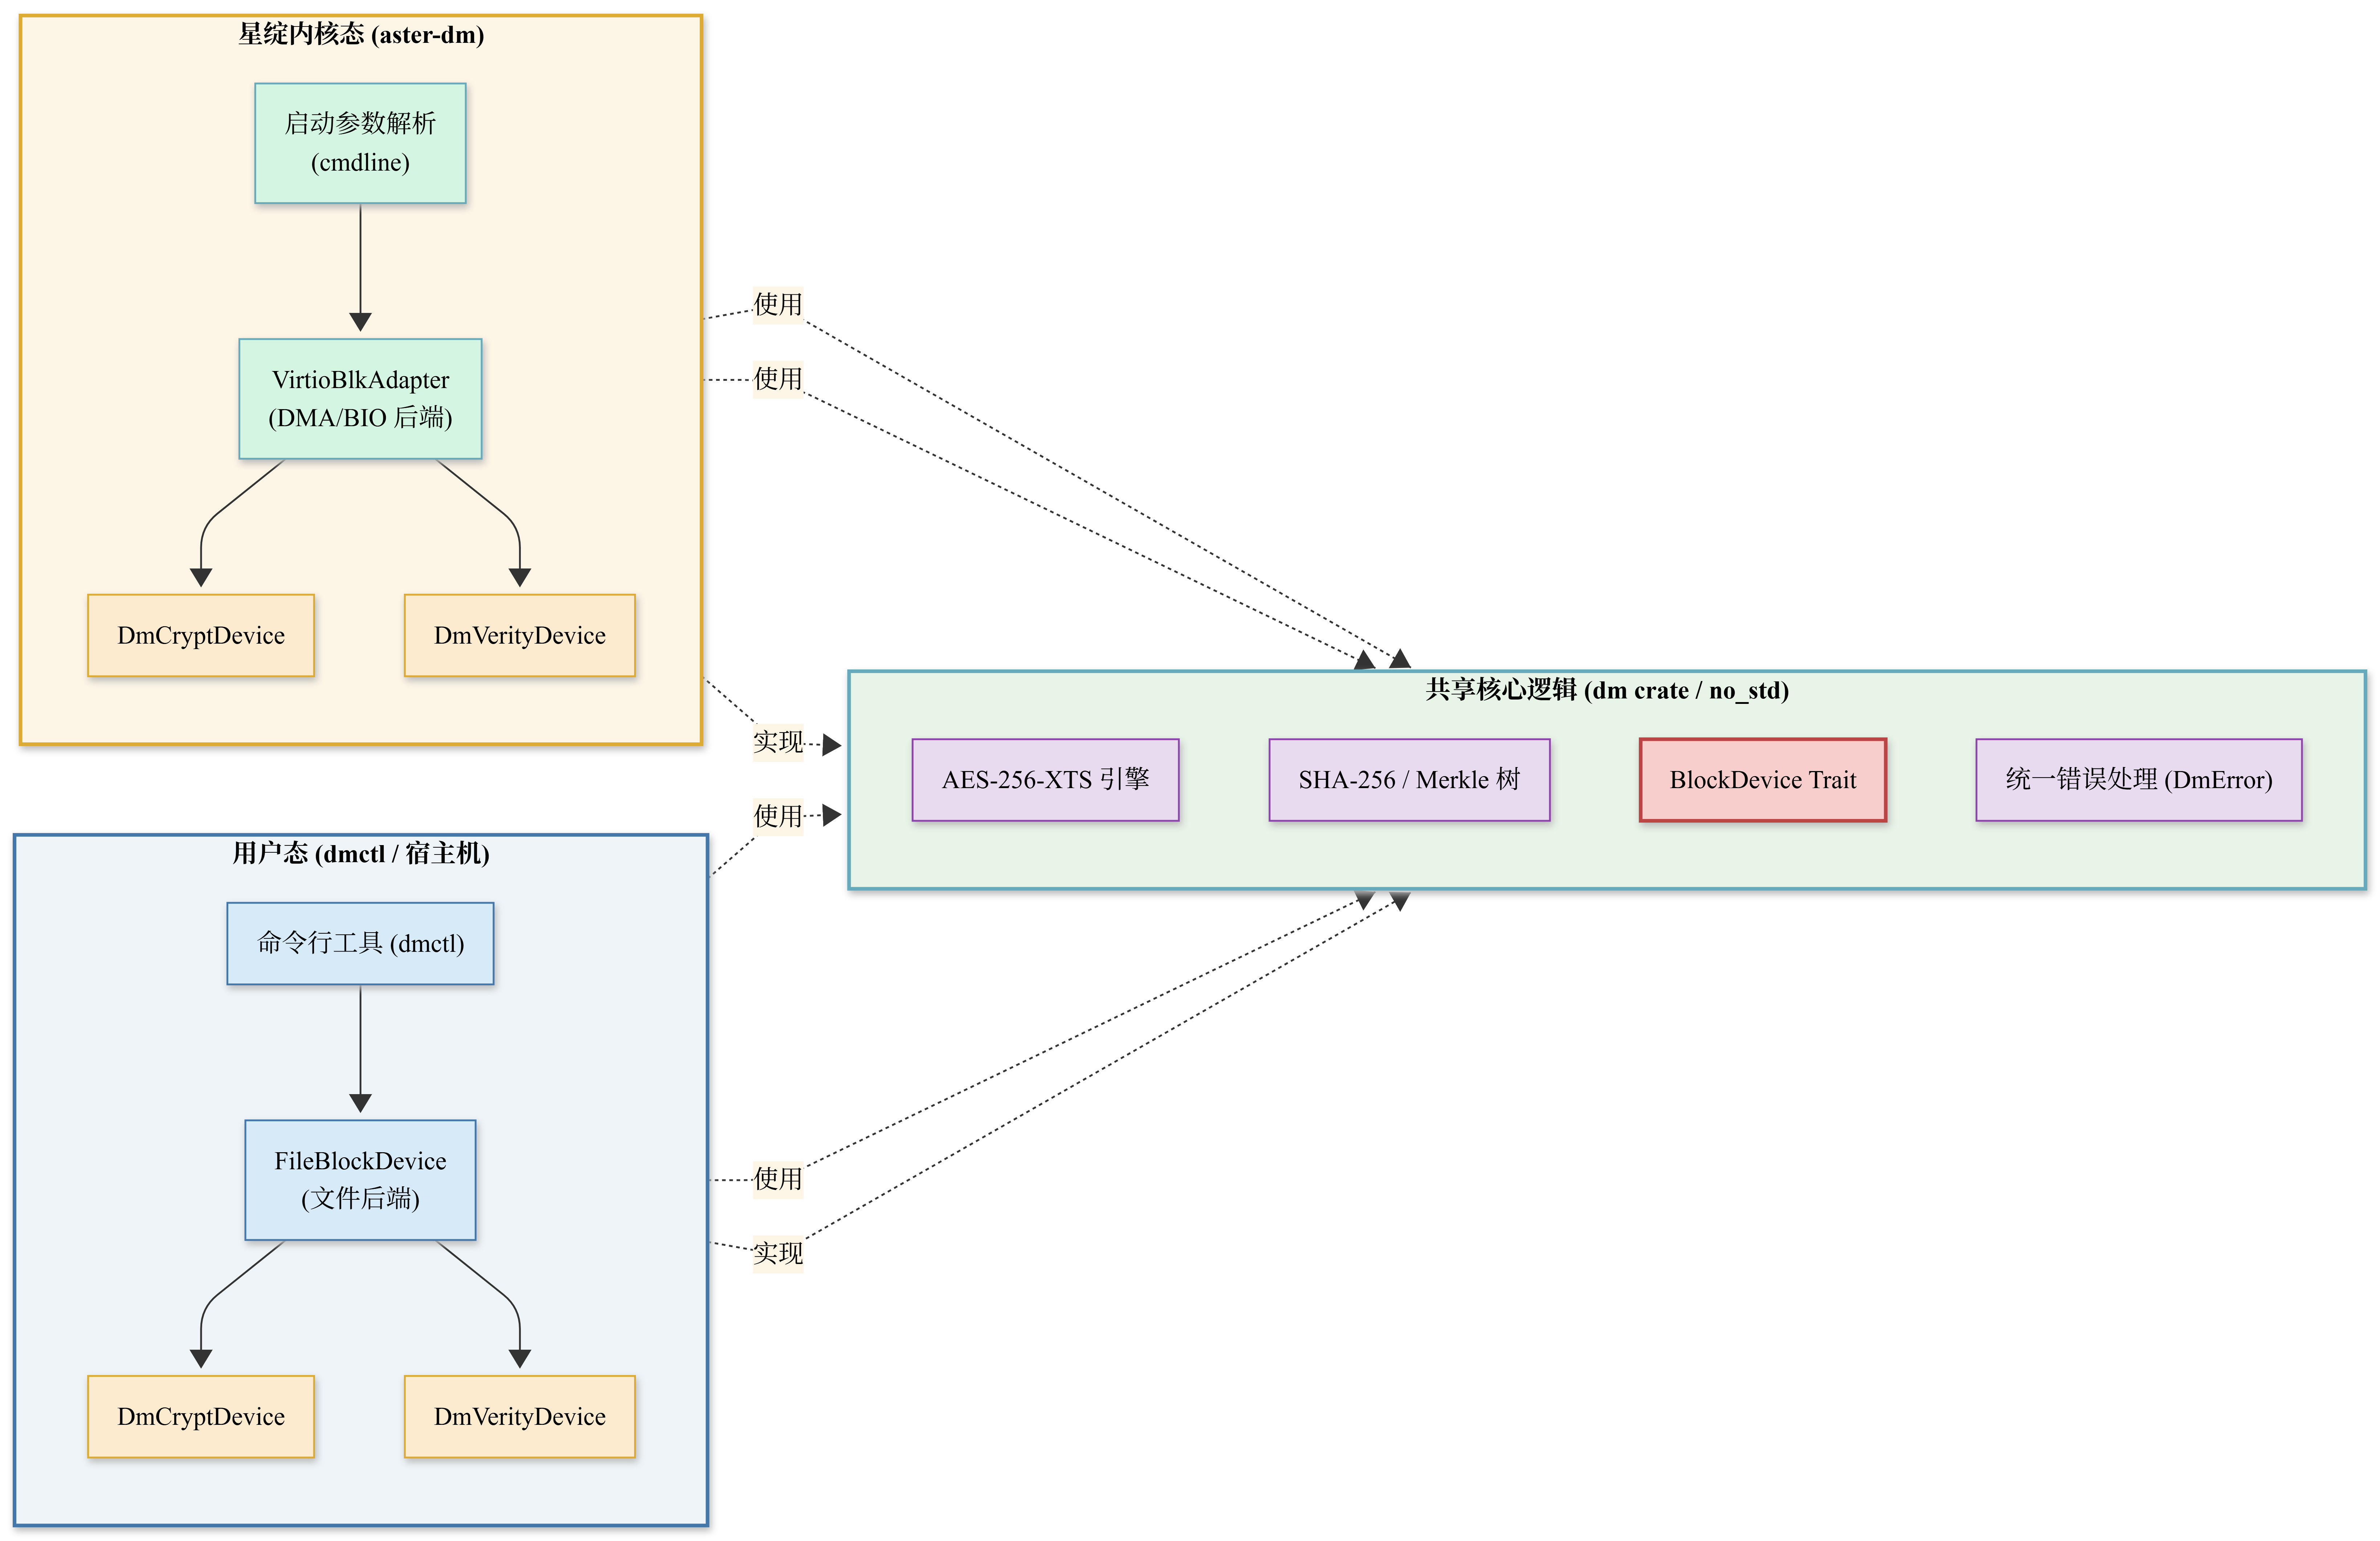
\includegraphics[width=0.95\textwidth]{code_entity_mapping_userspace_kernel.png}
    \caption{代码实体映射图（用户态 vs 星绽内核）}
    \label{fig:code_entity_mapping}
\end{figure}

如上图所示，用户态和内核态共享同一套核心算法实现（AES-XTS、SHA-256、Merkle 树验证），但适配层完全隔离：

\begin{itemize}
    \item \textbf{用户态}：\texttt{dmctl} 工具实例化一个 \texttt{FileBlockDevice}，并根据命令行参数将其包装在 \texttt{DmCryptDevice} 或 \texttt{DmVerityDevice} 中；所有 I/O 操作是同步的，使用 \texttt{std::sync::Mutex} 保证线程安全。
    \item \textbf{内核态}：在星绽中，\texttt{VirtioBlkAdapter} 包装了内核内部的块设备句柄。由于该适配器实现了 \texttt{BlockDevice}，\texttt{DmCryptDevice} 可以无需任何修改地直接包装它；I/O 操作是异步的（BIO），使用 \texttt{spin::Mutex} 和原子操作保证并发安全，在 AES-NI 变换期间还须通过 \texttt{disable\_preempt} 和 \texttt{irq::disable\_local} 保护 XMM 寄存器。
    \item \texttt{no\_std} 兼容性：核心 \texttt{dm} 库设计为最小化依赖（例如，\texttt{aes} crate 设置 \texttt{default-features = false}），以促进在可能限制标准库的内核环境中执行。
\end{itemize}

代码实体映射关系如下：

\begin{table}[H]
    \centering
    \caption{用户态与内核态实体映射}
    \begin{tabular}{p{0.22\textwidth}p{0.33\textwidth}p{0.35\textwidth}}
        \toprule
        \textbf{功能} & \textbf{用户态（dmctl）} & \textbf{内核态（aster-dm）} \\
        \midrule
        代码 & \texttt{crates/dm/}、\texttt{crates/dmctl/} & \texttt{asterinas/kernel/comps/dm/}，补丁 \texttt{asterinas\_port/patches/} 0001--0007 \\
        块设备后端 & \texttt{FileBlockDevice} / \texttt{MemoryBlockDevice} & \texttt{VirtioBlkAdapter}（virtio-blk BIO） \\
        加密映射器 & \texttt{DmCryptDevice} & \texttt{DmTarget::Crypt} \\
        完整性映射器 & \texttt{DmVerityDevice} & \texttt{DmTarget::Verity} \\
        组合构建器 & \texttt{DmStackBuilder} / \texttt{demo-stack} & \texttt{dm\_stack=crypt,verity}（补丁 0007） \\
        控制接口 & 命令行、\texttt{crypt-table-fill} & \texttt{/dev/mapper/control}（供 cryptsetup） \\
        同步 & \texttt{std::sync::Mutex} & \texttt{spin::Mutex} + \texttt{disable\_preempt} \\
        \bottomrule
    \end{tabular}
\end{table}

\section{数据流架构}

下图展示了应用程序的 I/O 请求如何穿过该分层栈：

\begin{figure}[H]
    \centering
    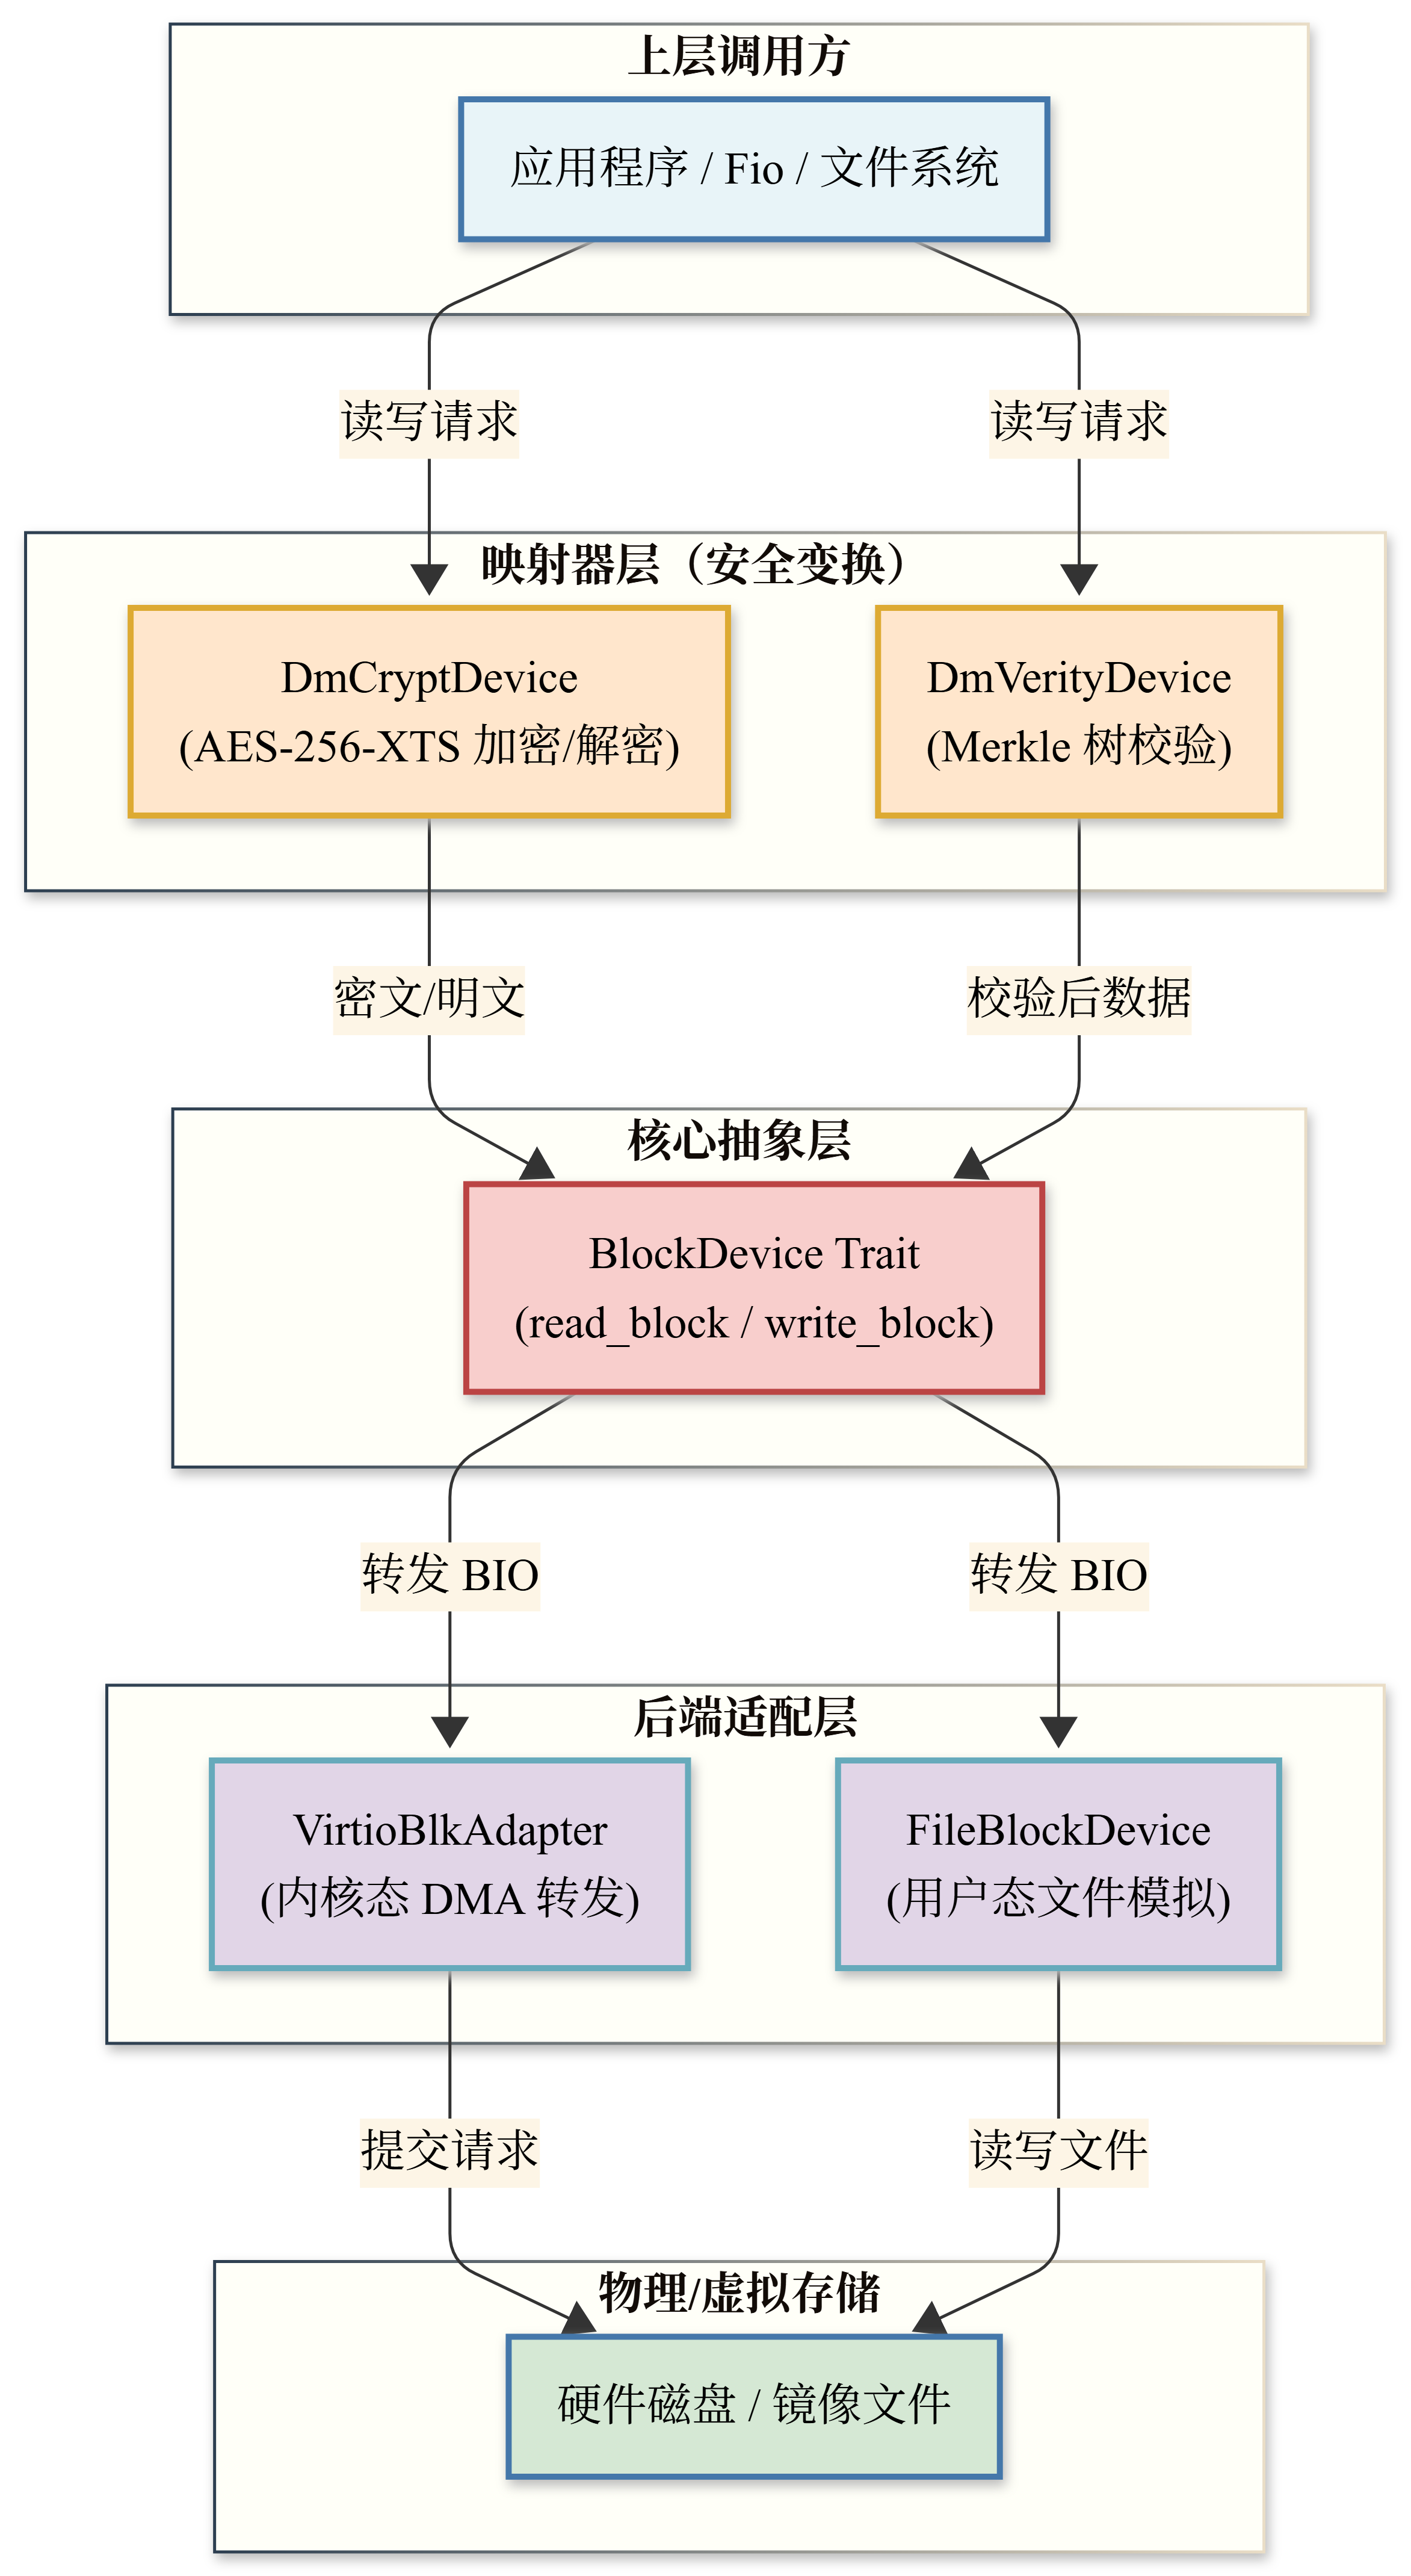
\includegraphics[width=0.9\textwidth]{block_io_layered_stack.png}
    \caption{块 I/O 分层栈数据流图}
    \label{fig:io_stack}
\end{figure}

在此模型中，\texttt{DmCryptDevice} 在执行 AES-256-XTS 转换后，将生成的密文传递给链中的下一个设备。类似地，\texttt{DmVerityDevice} 拦截读请求，以根据 Merkle 树校验数据的完整性。

\subsection{dm-crypt 数据流}

\textbf{写入路径}：按块号算扇区 $\to$ scratch 缓冲 $\to$ AES-XTS（扇区号作 plain64 IV）$\to$ 下层设备。4 KiB 块拆成 8 个 512 字节扇区分别变换，才能和 Linux 一致。具体步骤：

\begin{enumerate}
    \item 应用程序或文件系统向 \texttt{DmCryptDevice} 发起 \texttt{write\_block} 请求；
    \item 根据逻辑块 ID 和 \texttt{iv\_offset} 计算对应的物理扇区号；
    \item 从 scratch pool 获取临时缓冲区，调用 \texttt{Aes256XtsCipher} 对数据进行加密，使用扇区号作为 plain64 IV；
    \item 通过 \texttt{BioSegment::alloc\_bytes} 创建 bounce segment，将密文写入底层 \texttt{BlockDevice}；
    \item 底层设备完成写入后，释放 scratch 缓冲区，完成上层 BIO。
\end{enumerate}

\textbf{读取路径}是上述过程的逆操作：从底层设备读取密文到 scratch 缓冲区，使用相同的扇区号进行解密，然后写回上层 segment，最后释放 scratch 缓冲区。

\subsection{dm-verity 数据流}

\textbf{读取路径}：读数据块 $\to$ SHA-256 $\to$ 沿 on-disk 树或认证后缓存走到 root hash $\to$ 不一致则 \texttt{IntegrityViolation}。\textbf{写一律拒绝}。具体步骤：

\begin{enumerate}
    \item 从底层块设备读取原始数据块；
    \item \texttt{HashTree::verify\_block} 计算检索到的数据的 SHA-256 哈希值；
    \item 在每一层，从 on-disk 哈希树或认证后缓存中检索对应哈希值；
    \item 将重新计算出的哈希值与 \texttt{DmVerityDevice} 中存储的 root hash 进行比对；
    \item 如果哈希值不匹配，返回 \texttt{IntegrityViolation} 错误；若匹配且哈希块此前未缓存，则将其插入认证后缓存供后续复用。
\end{enumerate}

\section{线程安全保证}

所有后端均实现了 \texttt{Sync}，允许跨线程共享：

\begin{itemize}
    \item \texttt{MemoryBlockDevice}：在整个块向量周围使用 \texttt{Mutex}，确保安全性但将所有 I/O 串行化；
    \item \texttt{FileBlockDevice}：在 \texttt{File} 对象周围使用 \texttt{Mutex}，锁在 seek、read/write 和 flush 序列的整个持续时间内被持有；
    \item \texttt{PassthroughDevice}：依赖于底层设备实现了 \texttt{Sync}。
\end{itemize}

在星绽内核中，\texttt{DmDevice} 通过 \texttt{enqueue} 方法处理 BIO，内部使用 \texttt{spin::Mutex} 保护共享状态（如 \texttt{CryptScratchPool} 和 \texttt{VerifiedHashBlockCache}），并遵循内核的并发模型。内核态使用自旋锁而非睡眠锁的原因是——在 BIO 完成回调等中断上下文中不能睡眠，而自旋锁可以在禁用抢占和中断的情况下安全地持有，不会导致调度延迟或死锁。AES-NI 变换期间通过 \texttt{disable\_preempt} 和 \texttt{irq::disable\_local} 确保 XMM 寄存器不被中断上下文破坏——这是因为 AES-NI 指令使用 XMM 寄存器，而中断处理程序可能复用这些寄存器导致数据损坏。

\section{性能可观测性设计}

为了支持性能归因和优化验证，架构中集成了统计模块：

\begin{itemize}
    \item \texttt{InstrumentedDevice}：一个装饰器，可以插入到任意两层之间，记录读/写次数、字节数、失败次数以及累计和最大延迟（以纳秒计）；
    \item \texttt{IoStatsSnapshot}：提供稳定的快照，便于在基准测试前后对比；
    \item 在 Asterinas 内核中，通过启动参数 \texttt{dm.perf\_stats=1} 启用细粒度阶段计时（如 \texttt{lower\_wait}、\texttt{AES-XTS}、\texttt{SHA-256}、\texttt{cache\_lookup} 等），并通过 \texttt{\seqsplit{/proc/dm-performance-stats}} 导出；
    \item \texttt{/proc/dm-verity-stats} 提供 \texttt{verified}、\texttt{bio\_blocks}、\texttt{data\_rereads}、\texttt{hash\_hits}、\texttt{hash\_misses}、\texttt{auth\_shortcuts} 等计数器，直接反映优化效果——这些计数器在正式性能测试中用于验证 BIO 复用（\texttt{data\_rereads=0}）和缓存命中（\texttt{auth\_shortcuts}）的实际收益。
\end{itemize}

内核启用 \texttt{dm.perf\_stats=1} 后的实测归因数据表明：dm-crypt 热路径里下层等待约占 97.84\%、AES-XTS 约占 1.82\%；dm-verity 下层等待约占 93.01\%、数据 SHA-256 约占 5.74\%。算法本身不是主瓶颈，所以优化优先做缓冲池、缓存和 BIO 复用，而不是再改一轮 AES。

这种设计使得开发者可以精确量化每个映射器层的开销，从而指导优化方向。

\section{运行时控制面（Linux 兼容）}

为了支持 \texttt{cryptsetup} 等用户态工具，项目实现了与 Linux \texttt{dm\_ioctl} 兼容的控制接口：

\begin{itemize}
    \item \texttt{DmControlDevice}：在 \texttt{/dev/mapper/control} 提供 ioctl 处理，支持 \texttt{DM\_DEV\_CREATE}、\texttt{DM\_TABLE\_LOAD}、\texttt{DM\_DEV\_SUSPEND}、\texttt{DM\_DEV\_STATUS}、\texttt{DM\_DEV\_REMOVE} 等命令；
    \item \texttt{RuntimeMapper}：管理动态创建的 mapper，包括状态机（Empty、Loaded、Active）和密钥的清除——当 mapper 被删除时，未激活表中的密钥会被显式清零，防止密钥残留在内存中；
    \item 通过该接口，Asterinas 内核可以接受来自 \texttt{cryptsetup} 的标准 table 字符串，动态激活加密映射器，从而实现与 Linux 生态的互操作。
\end{itemize}

\section{安全能力传播}

\texttt{DmStackBuilder} 和 \texttt{DmStack} 提供安全能力的自动汇总：

\begin{lstlisting}[language=Rust, basicstyle=\ttfamily\small, breaklines=true]
pub struct TargetCapabilities {
    pub confidentiality: bool,
    pub integrity: bool,
    pub read_only: bool,
}
\end{lstlisting}

每个 target 声明自己提供的安全能力，最终栈通过 fold 操作自动汇总，使上层调用者可以静态获知组合后的安全属性。例如，\texttt{crypt + verity} 栈自动获得 \texttt{confidentiality=true}、\texttt{integrity=true}、\texttt{read\_only=true}。这种设计将安全策略的传播在编译期完成，避免了运行时动态检查的开销和遗漏风险。

\section{Asterinas 内核集成架构}

\texttt{aster-dm} 组件通过以下方式接入 Asterinas 内核：

\begin{enumerate}
    \item \textbf{组件声明}：在 \texttt{Components.toml} 中注册 \texttt{aster-dm}，在 \texttt{kernel/Cargo.toml} 中引入依赖；
    \item \textbf{启动参数解析}：使用 \texttt{aster-cmdline::define\_kv\_param!} 宏定义 \texttt{dm\_crypt.*}、\texttt{rootfs\_verity.*} 和 \texttt{dm\_stack} 参数；
    \item \textbf{块设备注册}：通过 \texttt{aster\_block::register} 将 mapper 注册为块设备，分配主设备号和次设备号；
    \item \textbf{BIO 处理}：在 \texttt{BlockDevice::enqueue} 中根据 \texttt{DmTarget} 类型分发到对应的处理函数（\texttt{process\_crypt}、\texttt{process\_verity}），所有 I/O 操作均通过 BIO 异步提交；
    \item \textbf{根切换}：initramfs 中的 \texttt{init} 脚本在 \texttt{dm-root} 模式下挂载 mapper，执行 \texttt{pivot\_root} 切换到受保护根。
\end{enumerate}

补丁序列（\texttt{asterinas\_port/patches/0001--0007}）记录了完整的集成演进历史，每一补丁对应一个可独立验证的增量功能，总补丁代码量约 4000 行。补丁用法详见 \texttt{asterinas\_port/README.md}。

\section{小结}

本章详细阐述了系统的核心架构，包括统一的 \texttt{BlockDevice} 抽象、可组合的映射器链模式、模块分解（含约行数）、双目标跨环境可移植性（含代码实体映射表）、数据流架构（含 4 KiB 拆 8 扇区的关键约束和 verity 写拒绝语义）、线程安全保证（含内核/用户态锁策略差异）、性能可观测性设计（含实测归因百分比）、运行时控制面、安全能力传播和 Asterinas 内核集成架构。

关键设计亮点回顾：
\begin{itemize}
    \item \texttt{BlockDevice} trait 作为统一抽象，支撑了整个存储安全框架；
    \item 双目标架构使用户态可作为"安全网"快速验证算法，内核态才是赛题交付物；
    \item Rust 的类型系统（\texttt{Send}、\texttt{Sync}、\texttt{TargetCapabilities}）在编译期保证了线程安全和安全能力传播的正确性；
    \item 性能归因数据表明算法本身不是主瓶颈，优化优先做缓冲池、缓存和 BIO 复用；
    \item 性能可观测性设计将优化决策建立在量化数据之上，而非经验猜测。
\end{itemize}

在接下来的章节中，我们将深入探讨 \texttt{dm-crypt} 和 \texttt{dm-verity} 的具体实现细节，以及如何将上述框架设计落地为可运行的代码。
